\documentclass[format=sigconf]{acmart}
\usepackage{minted}
\usepackage{xcolor}
\usepackage{xspace}
\usepackage[utf8]{inputenc}
\usepackage[T1]{fontenc}
\usepackage{amsmath}
\usepackage{amssymb}
\usepackage{graphicx}
\usepackage{varioref}   %
\usepackage{hyperref}
\usepackage[nameinlink,capitalize]{cleveref}
\usepackage{tocloft}
\usepackage{amsthm} % example env
\usepackage{enumitem} % description env
\usepackage{tikz}

\newcommand\asterism{\medskip\noindent\textcolor{black!65}{\small\centerline{$\phantom{x}_{*\,\,\,*}^{\,\,\,*}$}}\smallskip}

\usemintedstyle{xcode}
\newminted{cl}{autogobble,breaklines,escapeinside=||,fontsize=\small}

\newcommand\code[2][\small]{\sloppy\texttt{#1#2}}
\newcommand\footcode[1]{\code[\scriptsize]{#1}}

\theoremstyle{definition}
\newtheorem{example}{Example}

\usetikzlibrary{positioning,shapes,shadows}


\bibliographystyle{alpha}

\acmConference[ELS'19]{the 19th European Lisp Symposium}{April 01--02 2018}{Genova, Italy}
\acmISBN{978-2-9557474-2-1}
\acmDOI{}

\title{Implementing Baker's SUBTYPEP decision procedure}

\author{Léo Valais}
\email{lvalais@lrde.epita.fr}
\orcid{0000-0000-0000-0000}

\author{Jim E. Newton}
\email{jnewton@lrde.epita.fr}
\orcid{0000-0002-1595-8655}

\author{Didier Verna}
\email{didier@lrde.epita.fr}
\orcid{0000-0002-6315-052X}

\affiliation{%
  \institution{EPITA/LRDE}
  \streetaddress{14-16 rue Voltaire}
  \postcode{94270}
  \city{Le Kremlin-Bic{\^e}tre}
  \country{France}
}

\begin{CCSXML}
  <ccs2012>
  <concept>
  <concept_id>10011007.10011006.10011008.10011024.10011028</concept_id>
  <concept_desc>Software and its engineering~Data types and structures</concept_desc>
  <concept_significance>500</concept_significance>
  </concept>
  <concept>
  <concept_id>10003752.10003790.10011740</concept_id>
  <concept_desc>Theory of computation~Type theory</concept_desc>
  <concept_significance>500</concept_significance>
  </concept>
  <concept>
  <concept_id>10003752.10003809.10010031.10010032</concept_id>
  <concept_desc>Theory of computation~Pattern matching</concept_desc>
  <concept_significance>300</concept_significance>
  </concept>
  </ccs2012>
\end{CCSXML}

\ccsdesc[500]{Software and its engineering~Data types and structures}
\ccsdesc[500]{Theory of computation~Type theory}
\ccsdesc[300]{Theory of computation~Pattern matching}


\newcommand\sbcl{\textsc{Sbcl}}
\newcommand\then{$\rightarrow$}

\begin{document}


% \toappear{}
\begin{abstract}
  The Common Lisp standard allows the function \code{subtypep} to return
  the couple of values \code{(nil nil)} when it cannot determine the
  sub-typing relationship between two types. That permission to fail
  is granted because the type system allows the usage of the type specifier
  \code{(satisfies P)}, understood as the type containing all the
  elements for which the predicate \code{P} return $\top$. Since \code{subtypep}
  must not evaluate \code{P}, it cannot answer many interrogations involving
  such a type specifier---hence the permission to fail. Implementations of the
  predicate often abuse such permission, making the function both inaccurate and
  unreliable. That behavior is troublesome for some applications, in particular
  for the compiler itself which uses \code{subtypep} for optimization purposes.
  Seeking for precision, H. Baker describes a decision procedure which he claims
  to be more accurate and efficient than the average implementation.
  In this article we present our partial implementation of his procedure, detail
  our understanding of his algorithm, argument in favor or against some of
  his choices and clarify parts of his description.
\end{abstract}

\maketitle

\section{Introduction}
The Common Lisp standard \cite{bib:ansi.94.cl} provides the predicate function
\code{subtypep} for
introspecting the sub-typing relationship. Every invocation \code{(subtypep A B)}
either returns the values \code{(t t)} when \code{A} is a sub-type of \code{B},
\code{(nil t)} when not or \code{(nil nil)} meaning the predicate could not
(or failed to) answer the question. The latter can happen when the type
specifier \code{(satisfies P)} (representing the type $\{x \mid
\mathtt{P(x)}\}$ for some predicate and total function\footnote{A function
  defined over its entire definition domain.} \code{P}) is involved. As shown in
\vref{lst:satisfies}, there is indeed no way for the function to answer anything
else than \code{(nil nil)} for any arbitrary predicates \code{F} and \code{G}.

However some implementations abuse of the permission to return \code{(nil nil)}.
For example, in \sbcl{} (the implementation we are currently focusing our
efforts on), {\small\code{(satisfies 'boolean 'keyword)}} returns
\code{(nil nil)}, thus violating the standard\footnote{The Common Lisp standard
  requires that no invocation of \footcode{subtypep} involving only primitive types
  returns \footcode{(nil nil)}.}. The definition of the \code{keyword} type is
responsible for the failure: as shown in \vref{lst:keyword}, it
involves a \code{satisfies} type specifier. Therefore any type-based
optimization involving determining whether \code{boolean} is a sub-type of
\code{keyword} is lost.

Another kind of problem for which \code{subtypep}'s accuracy matters is the
optimization of the \code{typecase} construct as shown in \cite{newton.18.phd}
and \cite{newton.18.els}. The aim is to remove redundant checks in the construct
and their approach is to use binary decision diagrams. However, to build such a
structure, \code{subtypep} is repeatedly used. The unreliability of the
predicate leads here to many lost BDD reductions and therefore to the
generation of sub-optimal code.

Our implementation is still in active development, currently targets
\sbcl{} and focuses almost entirely on results accuracy. It supports
\emph{primitive} types, \emph{user-defined} types (\code{deftype}, classes and structures),
\emph{\code{member} (and \code{eql})} type specifiers and \emph{ranges} (e.g.,
\code{(integer * 12)}). We will present our strategy for implementing each one
of these while discussing how and why we decided or not to diverge from Baker's
\cite{baker1992}
approach---or potentially filling some gaps or unclear bits.
No optimization work has been done yet and the implementation still has
bugs and diverse issues but we have found some encouraging results about
accuracy and even about efficiency.

\begin{listing}[!p]
\begin{clcode}
(subtypep '(satisfies F) '(satisfies G))
;; returns (NIL NIL)
\end{clcode}
  \caption{Impossible for \code{subtypep} to answer}
  \label{lst:satisfies}
\end{listing}

\begin{listing}
  \begin{clcode}
(sb!xc:deftype keyword ()
  '(and symbol (satisfies keywordp)))
  \end{clcode}
  \caption{The \code{keyword} type definition in \sbcl}
  \label{lst:keyword}
\end{listing}


\section{The Common Lisp type system}
\subsection{Type specifiers}
We can equivalently speak of types and sets and Common Lisp types are no
exception. They are not manipulated directly. Instead, the type to be
manipulated is \emph{described} using a \emph{type specifier}.
The type specifier DSL (Domain-Specific Language) allows the programmer to
describe types by writing S-expressions which obey some rules described in the
Common Lisp standard \cite{bib:ansi.94.cl} and roughly summarized by the
\vref{tab:ts}\footnote{More type specifiers exist. We do not describe them either
  because they are not implemented or because Baker's procedure ignores them as well.}.

A subtlety about this mechanism is that \emph{different type specifiers} can
represent the same type (e.g., \code{integer}, \code{(integer * *)} and
\code{(or fixnum bignum)} all describe the same type). It means that
\emph{symbolic computation does not suffice} to answer the sub-typing question.
As shown in \vref{lst:type=}, one could write a predicate, say \code{type=}, to
determine whether two type specifiers describe in fact the same type using
\code{subtypep}.

It is possible to define \emph{parametric aliases} using the \code{deftype}
construct. It is then possible to refer to a whole type specifier using its
alias. The \vref{lst:deftype} shows an example of parametric \code{deftype}.

\begin{listing}
\begin{clcode}
(defun type= (type1 type2)
  (multiple-value-bind (res1 sure1-p)
      (subtypep type1 type2)
    (multiple-value-bind (res2 sure2-p)
        (subtypep type2 type1)
      (values (and res1 res2)
              (and sure1-p sure2-p)))))
\end{clcode}
\caption{The predicate \code{type=}}
\label{lst:type=}
\end{listing}

\begin{listing}
\begin{clcode}
(deftype except (x)
  `(not (eql ,x)))
\end{clcode}
\caption{The \code{deftype} construct}
\label{lst:deftype}
\end{listing}

\begin{table*}
  \centering
  \newcommand\var[1]{{\color{gray}$#1$}}
  \newcommand\pat[1]{\texttt{\small #1}}
  \begin{tabular}{rl|c}
    \hline
    Type specifier pattern & Description & Example \\
    \hline
    \pat{nil} & The null type $\emptyset$ & --- \\
    \pat{\var{t}}
            & A \code{symbol}-designated type & \code{character} \\
    \pat{(eql \var{e})}
            & The singleton type $\{e\}$ & \code{(eql 12)} \\
    \pat{(member \var{e_1} $\cdots$ \var{e_n})}
            & The type $\{e_1, \cdots, e_n\}$ & \code{(member t nil)} \\
    \pat{(not \var{t})}
            & The complement type $\overline{t}$ & \code{(not null)} \\
    \pat{(or \var{t_1} $\cdots$ \var{t_n})}
            & The union type $t_1 \cup \cdots \cup t_n$ & \code{(or integer float)} \\
    \pat{(and \var{t_1} $\cdots$ \var{t_n})}
            & The intersection type $t_1 \cap \cdots \cap t_n$ & \code{(and symbol (not keyword))} \\
    \pat{(\var{t} \var{X} \var{Y})}
            & The range $\{n \in t \mid X \leq n \leq Y\}$ & \code{(integer 1 6)} \\
    \pat{(\var{t} (\var{X}) \var{Y})}
            & The range $\{n \in t \mid X < n \leq Y\}$ & \code{(integer (0) 6)} \\
    \pat{(\var{t} * (\var{Y}))}
            & The range $\{n \in t \mid n < Y\}$ & \code{(integer * (43))} \\
    \pat{(array \var{t} \var{n})}
            & $n$-dimensional array of elements of type $t$ & \code{(array integer 1)} \\
    \pat{(array * (\var{d_1} $\cdots$ \var{d_n}))}
            & Array with $d_i$ elements in its $i$-th dimension & \code{(array * (3 3))} \\
    \pat{(array \var{t} (* * *))}
            & 3-dimensional $t$ array & \code{(array symbol (* * *))} \\
    \pat{(satisfies \var{p})} & The type $\{x \mid p(x)\}$ & \code{(satisfies oddp)} \\
    \hline
  \end{tabular}
  \caption{Brief summary of the type specifier DSL features}
  \label{tab:ts}
\end{table*}

\subsection{Vocabulary}
Follows some vocabulary, notations and conventions used in this article.

\begin{description}[leftmargin=8em,style=nextline]
  \item[type] For any type $t$: $t \equiv \{x \mid x\!:\!t\}$
  \item[canonical t.s.] A type specifier without aliases.
  \item[primitive type] A standardized type that is not necessarily
    implemented as a class.
  \item[symbolic form] A type specifier which type is \code{symbol}.
  \item[compound form] A type specifier which type is \code{list}.
  \item[logic type] A toplevel union, intersection or complement.
  \item[literal type] A type specifier that only contains symbolic types,
    \code{member} types and logic compound forms.
  \item[interval] A mathematical interval that may not be a valid type specifier.
  \item[range type] A type specifier that only contains ranges and logic compound forms.

  \item[type $\approx$ t.s.] When no confusion is possible we take the right to
    write type specifiers where a mathematical type is expected and to use a type
    variable, say $T$, as a placeholder inside Lisp code for \emph{a type
      specifier describing} $T$.
  \item[$T \subseteq T'$] The \emph{type} $T$ is a non-strict sub-type of $T'$.
    We always have \code{(subtypep $T$ $T'$)}.
  \item[$T \subset T'$] The \emph{type} $T$ is a strict sub-type of $T'$.
    We always have \code{(and (subtypep $T$ $T'$) (not (subtypep $T'$ $T$)))}.
\end{description}

\section{General procedure flow}
\label{sec:flow}
\vref{fig:flow} pictures the internals of our implementation. Every step will be
detailed in the following sections. There is three \emph{major stages}:

\begin{enumerate}
\item \emph{The preprocessing} --- Both type specifiers are processed in order to
  simplify further calculations: the aliases are expanded, each occurrence of
  numeric types are converted to their equivalent range type specifier and the
  type specifier is finally splitted. This stage is detailed in % section
  \vref{sec:pre}.
\item \emph{Expert sub-procedures} --- Once splitted, each sub-type specifier is
  redirected to the appropriate expert sub-procedure. Such procedures' job is to
  determine, in its own \emph{kingdom} in Baker's terminology, whether or not it
  can \emph{prove} the assertion ``$A$ is a sub-type of $B$'' to be \emph{wrong}.
  Our procedures currently only supports literal and range type specifers---an
  expert sub-procedure has been implemented only for these two kingdoms. This
  stage is detailed in \vref{sec:exp}.
\item \emph{Result accumulation} --- Eventually, all expert sub-procedures
  return (a boolean) and the results are accumulated using conjunction.
  From a top-down point of view, the \code{subtypep} function could be
  implemented as shown in \vref{lst:tdstp}.
\end{enumerate}

\begin{listing}
\begin{clcode}
(defun subtypep (a b)
  (reduce (lambda (x y) (and x y))
          (mapcar (lambda (expert t1 t2)
                    (funcall expert t1 t2))
                  (list #'literal-sub-proc #'range-sub-proc)
                  (split (num-types->ranges (expand a)))
                  (split (num-types->ranges (expand b))))))
\end{clcode}
\caption{A top-down approach of \code{subtypep}}
\label{lst:tdstp}
\end{listing}

\begin{figure}
  \centering
  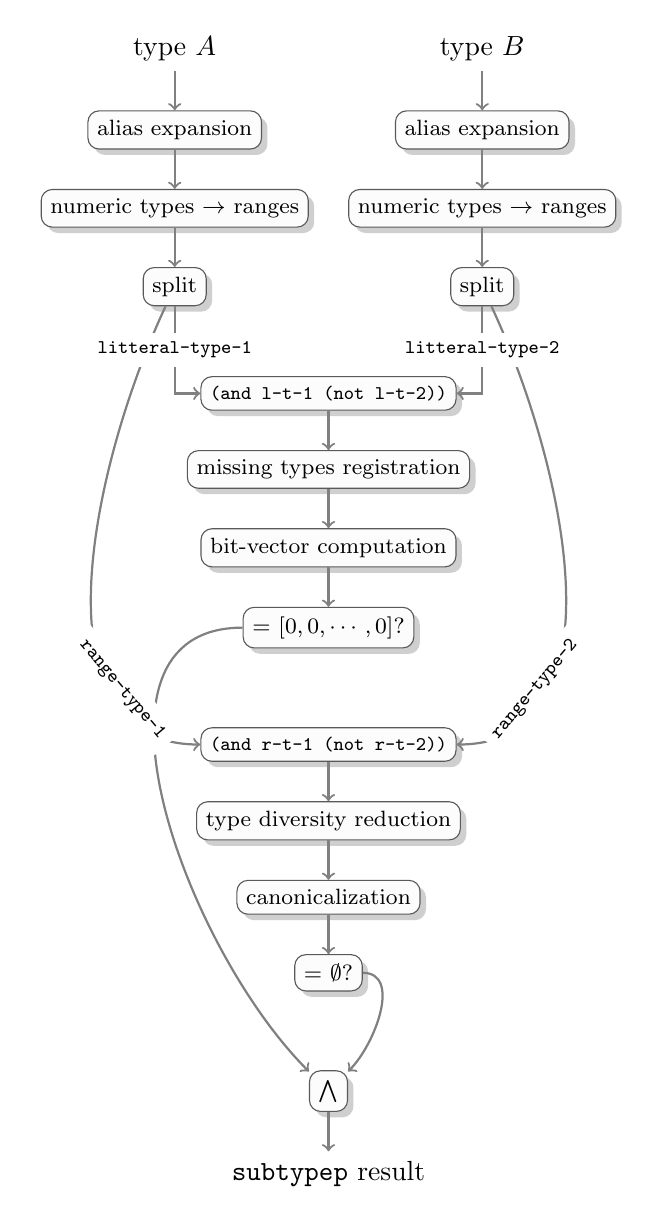
\begin{tikzpicture}[node distance=5mm,
  action/.style={rectangle,rounded corners,fill=white,drop shadow=gray!75,draw=black!65,fill=gray!2,font=\footnotesize},
  andnot/.style={action,font=\scriptsize\tt},
  arrow/.style={->,thick,gray},
  label/.style={fill=white,text=black,font=\tt\scriptsize},
  inout/.style={}
  ]
  \def\longest{numeric types \then{} ranges}

  \node[action] (largest1) {\longest};
  \node[action,right=of largest1] (largest2) {\longest};
  \node[action,above=of largest1] (typexpand1) {alias expansion};
  \node[action,above=of largest2] (typexpand2) {alias expansion};
  \node[action,below=of largest1] (split1) {split};
  \node[action,below=of largest2] (split2) {split};
  \node[inout,above=of typexpand1] (a) {type $A$};
  \node[inout,above=of typexpand2] (b) {type $B$};
  \draw[arrow,opacity=0] (largest1) -- (largest2) node[midway,opacity=0] (middle) {};

  \node[andnot,below=2 of middle] (andnotL) {(and l-t-1 (not l-t-2))};
  \node[action,below=of andnotL] (reg) {missing types registration};
  \node[action,below=of reg] (bv) {bit-vector computation};
  \node[action,below=of bv] (nullbv) {= $[0,0,\cdots,0]$?};

  \node[andnot,below=1 of nullbv] (andnotR) {(and r-t-1 (not r-t-2))};
  \node[action,below=of andnotR] (red) {type diversity reduction};
  \node[action,below=of red] (canon) {canonicalization};
  \node[action,below=of canon] (nullin) {= $\emptyset$?};

  \node[action,below=1 of nullin] (conj) {$\bigwedge$};
  \node[inout,below=of conj] (res) {\texttt{subtypep} result};


  \draw[arrow] (a) to (typexpand1);
  \draw[arrow] (b) to (typexpand2);
  \draw[arrow] (typexpand1) to (largest1);
  \draw[arrow] (typexpand2) to (largest2);
  \draw[arrow] (largest1) to (split1);
  \draw[arrow] (largest2) to (split2);

  \draw[arrow] (split1) to [out=245,in=180] (andnotR);
  \draw[arrow] (split2) to [out=295,in=0] (andnotR);
  % near start = pos=0.1
  \draw[arrow] (split1) |- (andnotL) node[label,near start] (lt1) {litteral-type-1};
  \draw[arrow] (split2) |- (andnotL) node[label,near start] (lt2) {litteral-type-2};

  \draw[arrow] (andnotL) to (reg);
  \draw[arrow] (reg) to (bv);
  \draw[arrow] (bv) to (nullbv);
  \draw[arrow] (andnotR) to (red);
  \draw[arrow] (red) to (canon);
  \draw[arrow] (canon) to (nullin);

  \draw[arrow] (nullbv) to [out=180,in=135] (conj);
  \draw[arrow] (nullin) to [out=0,in=45] (conj);
  \draw[arrow] (conj) to (res);

  % tricky labels to place
  \node[label,left=.41 of andnotR,rotate=-50] (rt1) {range-type-1};
  \node[label,right=.41 of andnotR,rotate=50] (rt2) {range-type-2};
\end{tikzpicture}

  \caption{Internal flow for \code{(subtypep $A$ $B$)}}
  \label{fig:flow}
\end{figure}

\section{Preprocessing}
\label{sec:pre}
% Both \code{subtypep} parameters are first pre-processed independently.
% TODO add MOP bib ref for finalized classes
\subsection{Alias expansion}
The very first step is to ensure that the type specifier is in its
\emph{canonical form}, that is, having all its aliases expanded. For example,
considering the type created in \vref{lst:deftype},
\code{(expand '(except 12))} should return \code{(not (eql 12))}.

Unlike for the macro expansion, the \code{deftype} expansion is not
standardized. Thus a solution must be found for each implementation
independantly. As our efforts are focused on \sbcl{} (yet), we discuss how we
implement the \code{expand} function for that compiler.

\sbcl's \code{subtypep} heavily relies on the function
\code{sb-kernel:specifier-type}, which does type expansion. It also does
type simplification---turning \code{(and integer string)} into
\code{nil}---which could have saved us some work. We hoped we could simplify
that function to make it compatible with Baker's algorithm while keeping the
\code{deftype} expansion and the range canonicalization work. However we found,
thanks to \cite{newton.18.phd} tools, that the function is responsible for most
of the work of \code{subtypep}, as shown in \vref{fig:specifiertype}
\footnote{The \footcode{cached-subtypep-caching-call} is just a memoizing wrapper
  around \sbcl's \footcode{subtypep} which is a bit more efficient than the raw
  implementation}.
Considering the lack of efficiency of that function and the fact that it would
not be trivial to simplify it to only keep the interresting bits, we decided to
stick to another, more cost-effective solution.

The function \code{sb-ext:typexpand} takes a type specfier and tries to expand
it (not recursively) and either returns the expansion result or the input type
specifier if it is not expandable. \code{(sb-ext:typexpand 'integer)} returns
\code{integer} since it is not a \code{deftype} alias whereas
\code{(sb-ext:typexpand '(except 12))} returns \code{(not (eql 12))}.
To expand a whole type specifier, it just needs to go through it, applying
\code{sb-ext:typexpand} on each list or atom. One subtlety though is that the
result of an expansion may itself be an alias to expand\footnote{Fortunately,
  \footcode{sb-ext:typexpand} also returns a boolean indicating whether or not
  an expansion happened.}.

\newcommand\ststpscale{0.5}
\begin{figure}
  \centering
  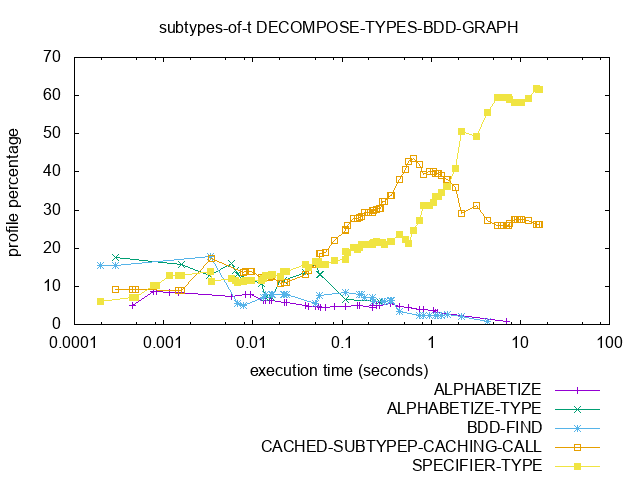
\includegraphics[scale=\ststpscale]{assets/19/stGTstp}
  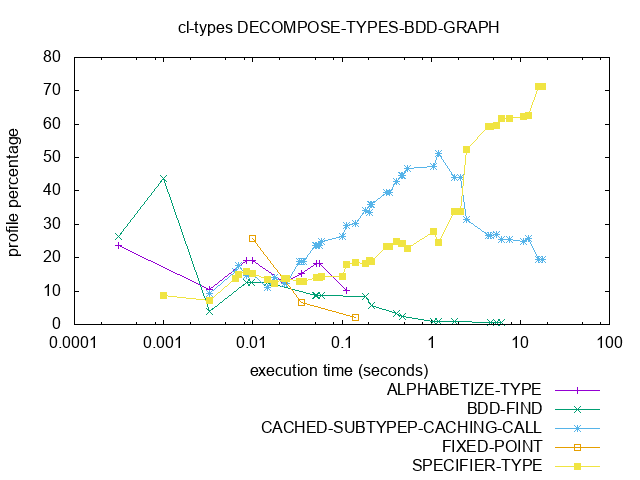
\includegraphics[scale=\ststpscale]{assets/19/stEQstp}
  \caption{\code{specifier-type} weight in \code{subtypep} execution}
  \label{fig:specifiertype}
  % \label{fig:stGTstp}
\end{figure}
%% NOTE perhaps separate the images in two distinct figures
% \begin{figure}
%   \centering
%   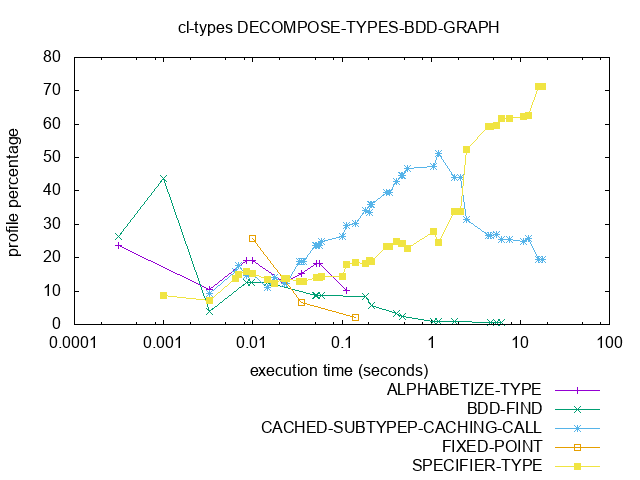
\includegraphics[scale=\ststpscale]{assets/19/stEQstp}
%   \caption{\code{specifier-type} weight in \code{subtypep} execution}
%   \label{fig:stEQstp}
% \end{figure}

\subsection{Numeric type specifiers conversion}
\label{sec:numconv}
As explained in \vref{sec:flow}, after preprocessing both type specifiers, the
procedure splits in two expert sub-procedures: one for literal type specifiers
and one for range type specifiers, because their internal representation differ.
Numeric types---types containing numbers (mathematically speaking)---can have
different representations: a \emph{symbol} (e.g., \code{fixnum}), a \emph{range}
(e.g., \code{(integer 1 6)}) or a \emph{\code{member} expression}
(e.g., \code{(member 1 2 3)}). However, the first two are literal where le
latter is a range. Thus, the numerical type information would be distributed in
the different expert sub-procedures (which does not share any data). For
consistency's sake and to obtain accurate results, a single internal
representation should be chosen. The symbolic and \code{member} numeric types
must then be converted into an equivalent type specifier involving only ranges
to describe numerical data.

\begin{itemize}
\item \emph{Symbolic} numeric type specifier --- say \code{U}, replace it by
  \code{(U * *)}\footnote{Implementations supporting the IEEE floating point
    raise many concerns with \footcode{-0.0}, $NaN$, $+\infty$ and $-\infty$.
    Baker explains in detail how to handle these cases, which our implementation
    (FIXME is that assertion totally true?)
    does not support yet.}. Note the new ``type specifier'' is likely
  \emph{not} to be valid (e.g., \code{(fixnum * *)} is invalid).
\item \code{member} type specifiers --- e.g., \code{(member a 1 2 :b)} is
  converted to \code{(or (member a :b) (bit 1 1) (integer 2 2))}.
  To do that,
  \begin{enumerate}
  \item extract the numbers out of the expression,
  \item map each number, say $n$, to construct the type specifier
    \code{((type-of $n$) $n$ $n$)}\footnote{\footcode{type-of} sometimes
      returns a list which \footcode{car} is the type of the range.},
  \item and combine the remaining \code{member} expression and the ranges with
    the \code{or} logic type specifier.
  \end{enumerate}
\end{itemize}

A subtlety to consider is that \textit{super-types} of \code{number} also
contain numerical data that must be extracted. Indeed, the type specifier
\code{atom} contains both numerical data---\code{(number * *)}---and non-numerical
data---\code{(and atom (not (number * *)))}. Unfortunately the latter
expression cannot be used since it uses the \code{atom} type specifier and
recursively converting that replacement would result in a infinite computation
loop. Thus \code{atom} must first be replaced by its sum type representation,
that is \code{(or stream array character function standard-object symbol
  structure-object structure-class (number * *))} before being recursively
converted. Similarly, the other super-type of \code{number}, the type \code{t}
must be replaced by \code{(or atom sequence)}.

Yet another subtlety is that the type specifiers \code{(and)} and
\code{(or)} respectively describe the types \code{t} and \code{nil}. Hence
every occurrence of \code{(and)} must be replaced by the replacement of
\code{t} described in the last paragraph. In order to remove that annoying
corner case completely, \code{(or)} is also replaced (by \code{nil}).

\subsection{Splitting}
Reached this step, the input only contains \emph{canonical} \emph{literal} and
\emph{range} type specifiers, numeric types being \emph{only} expressed as
ranges. The next stage---expert sub-procedures---requires literal and numeric
types to be separated.

Thus the top type \code{t} is divided into two\footnote{
  One per kingdom actually, but since out implementation only support
  two---literal and range types---we only focus our attention these.
} disjoint sub-types---``kingdoms'' as Baker says. The last step, described in
\vref{sec:numconv}, ensures the representation (in term of type specifiers) of
the types in each kingdom is different. All numeric types are represented as
ranges and literal types are represented as symbolic and \code{member} (without
numbers) type specifiers.

This step roughly consists in an in-depth traversal of the type specifier, using
pattern-matching to recognize which type specifier represents which type. We use
the implementation of \cite{bib:norvig.92.paip} for its simplicity and versatility.

Our implementation uses a function \code{type-keep-if} which takes a predicate
$P$ and a type specifier $T$ and returns:
\begin{itemize}
  \newcommand\mcode[1]{\text{\code{#1}}}
\item $T$ as it is when $P(T) = \top$,
\item \code{nil} when $P(T) = \bot$,
\item \code{($op$ $U_1$ $\cdots$ $U_n$)}
  where \(U_i = \mcode{(type-keep-if $P$ $T_i$)}\)
  when \(T = \mcode{($op$ $T_1$ $\cdots$ $T_n$)}\)
  and $op \in \{\mcode{and}, \mcode{or}, \mcode{not}\}$.
\end{itemize}
This function, given the predicate \code{literal-type-p} and a type $T$, returns
$T$ with every inner type specifier that describes a non-literal type
replaced by \code{nil} (interpreted as the \textit{empty type}). The result is then a
sub-type of \code{(and t (not number))}.
Likewise, given the predicate \code{range-type-p}, this function returns $T$
with every non-range inner type specifier replaced by \code{nil} (interpreted
this time as the \textit{empty range}). Thus the result is a sub-type of \code{number}.
Therefore, \code{split} can easily be implemented in terms of
\code{type-keep-if}, as shown in \vref{lst:split}.

\begin{listing}
\begin{clcode}
(defun split (type)
  (list (type-keep-if #'literal-type-p type)
        (type-keep-if #'range-type-p type)))
\end{clcode}
\asterism
\begin{clcode}
SLIME> (split 'symbol)
;; (SYMBOL NIL)
SLIME> (split '(ratio * *))
;; (NIL (RATIO * *))
SLIME> (split  '(and (or symbol (float * *) (ratio * *))
                     (not (not (number * *)))))
;; ((AND (OR SYMBOL NIL NIL) (NOT (NOT NIL)))
;;  (AND (OR NIL (FLOAT * *) (RATIO * *))
;;       (NOT (NOT (NUMBER * *)))))
\end{clcode}
\caption{The \code{split} function}
\label{lst:split}
\end{listing}

\subsection{Type unification}
According to theory, for any types $T$ and $U$,
\(T \subseteq U \Leftrightarrow T \cap \overline{U} = \emptyset\).
Therefore, for any type specifiers \code{T} and \code{U}, when
\code{(subtypep T U)} returns \code{T T}, then
\code{(subtypep `(and ,T (not ,U)) nil)} also returns \code{T T}.

The results of the \code{split} function are zipped together using
\code{(lambda (x y) `(and ,x (not ,y)))} before being passed to the expert
sub-procedures. This way, they will not have to prove that an arbitrary type is a
sub-type of \emph{another} arbitrary sub-type, but rather whether \emph{one}
arbitrary type specifier describes the empty type (which is substancially
easier to reason about and implement).

\section{Expert sub-procedures}
\label{sec:exp}

\section{Procedure for literal types}

\section{Conclusion and Future Work}
[..] (Flow programming @SICP)

Even if, in the future, we are to conclude that our implementation is less
efficient than those which already exists, Baker's algorithm would still likely to
improve the predicate's accuracy. Users would then have the ability to
choose whichever \code{subtypep} implementation fits their needs the best.

% Speak about https://lists.gnu.org/archive/html/gcl-devel/2005-07/msg00038.html
\bibliography{common}

\end{document}
